\documentclass[11pt,a4paper]{article}

\usepackage[utf8]{inputenc}
\usepackage[T1]{fontenc}
\usepackage{amsmath,amssymb,amsthm}
\usepackage{geometry}
\usepackage{booktabs}
\usepackage{xcolor}
\usepackage{physics}
\usepackage{graphicx}
\usepackage{hyperref}
\usepackage{enumitem}
\usepackage{caption}
\usepackage{tikz}
\usetikzlibrary{shapes,arrows.meta,positioning,calc,decorations.pathmorphing,decorations.markings}
\usepackage{orcidlink}
\usepackage{hyperref}
\hypersetup{colorlinks=true, linkcolor=blue, citecolor=blue, urlcolor=blue}

\geometry{margin=1in}

% Theorem environments
\newtheorem{theorem}{Theorem}[section]
\newtheorem{proposition}[theorem]{Proposition}
\newtheorem{lemma}[theorem]{Lemma}
\newtheorem{corollary}[theorem]{Corollary}
\theoremstyle{definition}
\newtheorem{definition}[theorem]{Definition}
\newtheorem{remark}[theorem]{Remark}
\newtheorem{axiom}{Axiom}

%==============================================================================
% QSD NOTATION (unified v3 — Hb/varsigma/varpi system)
%==============================================================================
% Holographic bit density
\newcommand{\Hb}{\textnormal{H\kern-0.3em b}}
\newcommand{\Hbn}{\Hb_n}
\newcommand{\Hbfour}{\Hb_4}
% Geometric strain
\newcommand{\strain}{\varsigma}
% Spectral bond
\newcommand{\specbond}{\varpi}
% Physics
\newcommand{\Esyn}{E_{\text{syn}}}
\newcommand{\Mpl}{M_{\mathrm{P}}}
\newcommand{\mH}{m_H}
\newcommand{\murad}{\mu_0}
\newcommand{\nurad}{\nu_0}
\newcommand{\Psyn}{P_{\text{syn}}}
\newcommand{\Punc}{P_{\text{unc}}}
\newcommand{\LL}{\mathcal{L}}
\newcommand{\aem}{\alpha_{\text{em}}}
\newcommand{\lp}{\ell_{\mathrm{P}}}

% Colors for diagrams
\definecolor{bulkcolor}{RGB}{70,130,180}
\definecolor{anchorcolor}{RGB}{220,20,60}
\definecolor{codegreen}{RGB}{0,128,0}
\definecolor{edgecolor}{RGB}{100,100,100}
\definecolor{u1color}{RGB}{34,139,34}
\definecolor{su2color}{RGB}{70,130,180}
\definecolor{su3color}{RGB}{200,50,50}

\title{
  \textbf{Quantum Spectrodynamics}:\\[0.5em]
  \Large Deriving Standard Model Parameters\\from the Geometry of Quantum Error-Correcting Codes\\[1em]
}

\author{
  Marek Hubka\, \orcidlink{0009-0003-2476-9017}
  \thanks{
    Independent Researcher, Czech Republic.\\
    Website: \href{http://www.tidesofuncertainty.com}{tidesofuncertainty.com}.\\
    Email: \href{mailto:marek@tidesofuncertainty.com}{marek@tidesofuncertainty.com}.
  }
}

\date{\today}

\begin{document}

\maketitle

\begin{abstract}
\noindent We present Quantum Spectrodynamics (QSD), a framework that derives Standard Model gauge couplings from a single structural input: the $[[5,1,3]]$ perfect quantum error-correcting code. The code determines two graphs -- the complete graph $K_4$ (bulk exchange interactions) and the cycle graph $C_5$ (geometric dynamics) -- from which three fundamental constants emerge: the holographic bit density $\Hbfour = 1/(4\ln 2)$, the geometric strain $\strain = 3/(80\varphi^2)$, and the spectral bond $\specbond = \pi\varphi^2$. From these, with zero free parameters, we derive:
the fine structure constant $\alpha^{-1} = 137.033$ (22~ppm),
the strong coupling $\alpha_s = 3\pi/80 = 0.1178$ (0.16\%),
and the weak mixing angle $\sin^2\theta_W = 3/13 + \strain/32 = 0.2312$ (within experimental error).
An exact algebraic identity $6\alpha_s = \alpha^{-1}_{\text{tree}} \times \Hbfour \times \strain$ connects the electromagnetic and strong sectors. We further derive the electroweak hierarchy $v_{\text{EW}}/\Mpl \sim 2^{-60}$ from the code state space and predict a syndrome energy $\Esyn = 28.24$~GeV consistent with reported LHC anomalies. The framework makes falsifiable predictions: if the 28~GeV feature reaches $5\sigma$ significance, QSD is ruled out.
The only experimental input is $\Mpl$. The only non-derived element is the specific functional form of $\strain$, whose individual factors are all code-determined but whose assembly is validated by predictions rather than proved from first principles.

\vspace{0.5em}
\noindent\textbf{Keywords:} quantum error correction, Standard Model, fine structure constant, strong coupling, information geometry, holographic principle
\end{abstract}

\tableofcontents
\newpage

%==============================================================================
\section{Introduction}
\label{sec:intro}
%==============================================================================

The Standard Model of particle physics is extraordinarily successful yet deeply incomplete. Its 19+ free parameters -- coupling constants, masses, mixing angles -- are measured with exquisite precision but remain unexplained. Why is $\alpha^{-1} \approx 137$? Why is $\alpha_s \approx 0.118$? Why is the Higgs mass 125~GeV~\cite{ATLASHiggs2012,CMSHiggs2012} rather than the Planck scale?

Quantum Spectrodynamics (QSD) proposes that these parameters are not free but are fixed by the structure of a quantum error-correcting code underlying spacetime. The connection between quantum information and spacetime geometry has deep roots: the Bekenstein--Hawking entropy formula \cite{Bekenstein1973,Hawking1975}, the holographic principle \cite{tHooft1993,Susskind1995}, and the discovery that quantum error correction provides the natural language for the bulk-boundary correspondence in AdS/CFT \cite{Almheiri2015,Pastawski2015} all point toward an information-theoretic foundation.

QSD takes this programme to its logical conclusion. If spacetime \emph{is} a quantum error-correcting code, then the parameters of low-energy physics should be determined by the code's mathematical structure. We show that the simplest perfect quantum code -- the $[[5,1,3]]$ code -- naturally produces the gauge groups, coupling constants, and mass hierarchy of the Standard Model.

\subsection{Summary of Results}

Starting from the single axiom that the vacuum is protected by a $[[5,1,3]]$ code, and with $\Mpl$ as the only experimental input, QSD derives:

\begin{table}[h]
\centering
\begin{tabular}{lccl}
\toprule
\textbf{Observable} & \textbf{QSD} & \textbf{Experiment} & \textbf{Accuracy} \\
\midrule
$\alpha^{-1}_{\text{em}}$ & $\mathbf{137.033}$ & 137.036 & 22~ppm \\
$\alpha_s(M_Z)$ & $\mathbf{0.11781}$ & $0.1180 \pm 0.0009$ & 0.16\% \\
$\sin^2\theta_W$ & $\mathbf{0.23122}$ & $0.23122 \pm 0.00003$ & $< 0.01\%$ \\
$\mH$ & $\mathbf{126.7}$~GeV & 125.1~GeV & 1.3\% \\
$\Esyn$ (syndrome) & $\mathbf{28.24}$~GeV & $\sim 28$~GeV$^*$ & 0.2\% \\
\bottomrule
\end{tabular}
\caption{QSD predictions vs.\ experiment. $^*$CMS dimuon anomaly \cite{CMS2018dimuon}. All values derived with zero free parameters.}
\label{tab:summary}
\end{table}

The framework also yields an exact algebraic identity connecting the electromagnetic and strong sectors, explains the electroweak hierarchy as an information-theoretic reduction factor, and makes falsifiable predictions for LHC Run~3.

\subsection{Epistemic Transparency}

We distinguish three categories throughout:
\begin{enumerate}[nosep]
    \item \textbf{Derived}: follows mathematically from the $[[5,1,3]]$ axiom (graphs, spectra, $\Hbfour$, $\specbond$).
    \item \textbf{Constructed}: every ingredient is derived, but the specific assembly is physically motivated rather than mathematically unique ($\strain$).
    \item \textbf{Open}: plausible but not yet rigorous (fermion mass hierarchy, CP violation).
\end{enumerate}
Complete proofs for all derived results are in Supplement~S1 \cite{Hubka2026QSDsupp}.

\subsection{Paper Organisation}

Section~\ref{sec:code} introduces the code foundation. Section~\ref{sec:graphs} develops the graph geometry. Section~\ref{sec:triad} derives the three fundamental constants. Section~\ref{sec:couplings} presents the gauge coupling predictions. Section~\ref{sec:hierarchy} derives the energy scale. Section~\ref{sec:action} presents the QSD action. Section~\ref{sec:pheno} covers phenomenology and falsification. Section~\ref{sec:open} discusses open problems. Appendix~\ref{app:notation} collects notation; Appendix~\ref{app:dct} maps QSD to Dimensional Collapse Theory.

%==============================================================================
\section{The $[[5,1,3]]$ Code Foundation}
\label{sec:code}
%==============================================================================

\subsection{The QSD Axiom}

\begin{axiom}[Code Structure]
\label{axiom:code}
The vacuum state of nature is protected by the $[[5,1,3]]$ quantum error-correcting code: 5 physical qubits encoding 1 logical qubit with distance 3.
\end{axiom}

The code is defined by four stabiliser generators with cyclic structure:
\begin{align}
g_1 &= X Z Z X I \\ 
g_2 &= I X Z Z X \\
g_3 &= X I X Z Z \\
g_4 &= Z X I X Z
\label{eq:stabilisers}
\end{align}
where $X$, $Z$ are Pauli matrices and $I$ is the identity. Each generator is obtained from the previous by a cyclic shift $i \to i+1 \pmod{5}$, reflecting the $\mathbb{Z}_5$ symmetry of the code.

The $[[5,1,3]]$ code is \emph{perfect}~\cite{Laflamme1996}: it saturates the quantum Hamming bound $2(1 + 3n) \leq 2^n$, which forces $n = 5$ as the unique solution. Every possible single-qubit error produces a unique syndrome, and no correction capacity is wasted.

\subsection{Why This Code?}

The choice of $[[5,1,3]]$ is not arbitrary. The quantum Hamming bound requires:
\begin{equation}
2^k(1 + 3n) \leq 2^n
\label{eq:hamming}
\end{equation}
For $k = 1$ (one logical qubit) and $d = 3$ (single-error correction), this gives $2(1 + 3n) \leq 2^n$. The unique solution is $n = 5$. This is an independent confirmation from standard quantum field theory: the Unruh effect~\cite{Unruh1976}  produces thermal noise (a depolarising channel) on the vacuum state, and the Hamming bound determines the minimal code that protects against it.

\begin{center}
\begin{tabular}{cccc}
\toprule
$n$ & LHS: $2(1+3n)$ & RHS: $2^n$ & Result \\
\midrule
3 & 20 & 8 & Impossible \\
4 & 26 & 16 & Impossible \\
\textbf{5} & \textbf{32} & \textbf{32} & \textbf{Saturates (perfect code)} \\
6 & 38 & 64 & Possible (but not minimal) \\
\bottomrule
\end{tabular}
\end{center}

\begin{theorem}[Minimal Vacuum Code]
The unique minimal quantum code that corrects arbitrary single-qubit errors on one logical qubit is $[[5,1,3]]$. It saturates the quantum Hamming bound with equality.
\end{theorem}

\subsection{Physical Interpretation}

The 5 physical qubits split into two groups:
\begin{itemize}[nosep]
    \item \textbf{4 bulk qubits} ($n - k = 4$ syndrome qubits): form the observable sector
    \item \textbf{1 anchor qubit} (the logical environment): the information boundary
\end{itemize}
The logical qubit protected by the code is identified with the Higgs field -- the unique scalar degree of freedom of the Standard Model.

%==============================================================================
\section{Graph Geometry: $K_4$ and $C_5$}
\label{sec:graphs}
%==============================================================================

The $[[5,1,3]]$ code determines two complementary graph structures.

\subsection{The Complete Graph $K_4$ (Bulk)}

When the anchor qubit is traced out, the remaining 4 bulk qubits interact via all possible pairwise channels. A code of distance $d = 3$ requires that any pair of bulk qubits can exchange error information, forcing the complete graph $K_4$.

\begin{figure}[h]
\centering
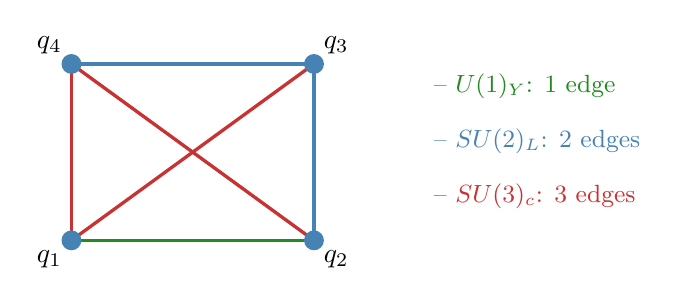
\begin{tikzpicture}[scale=1.4]
    % K4 vertices
    \coordinate (A) at (0,0);
    \coordinate (B) at (2.2,0);
    \coordinate (C) at (2.2,1.6);
    \coordinate (D) at (0,1.6);
    
    % Draw all 6 edges coloured by S4 irrep
    % U(1): 1 edge (green)
    \draw[u1color, very thick] (A) -- (B);
    % SU(2): 2 edges (blue)
    \draw[su2color, very thick] (B) -- (C);
    \draw[su2color, very thick] (C) -- (D);
    % SU(3): 3 edges (red)
    \draw[su3color, very thick] (D) -- (A);
    \draw[su3color, very thick] (A) -- (C);
    \draw[su3color, very thick] (B) -- (D);
    
    % Vertices
    \foreach \p in {A,B,C,D} {
        \fill[bulkcolor] (\p) circle (0.09);
    }
    
    % Vertex labels
    \node[below left] at (A) {$q_1$};
    \node[below right] at (B) {$q_2$};
    \node[above right] at (C) {$q_3$};
    \node[above left] at (D) {$q_4$};
    
    % Legend
    \node[anchor=west, font=\small] at (3.2,1.4) {\textcolor{u1color}{ --  $U(1)_Y$: 1 edge}};
    \node[anchor=west, font=\small] at (3.2,0.9) {\textcolor{su2color}{ --  $SU(2)_L$: 2 edges}};
    \node[anchor=west, font=\small] at (3.2,0.4) {\textcolor{su3color}{ --  $SU(3)_c$: 3 edges}};
\end{tikzpicture}
\caption{The complete graph $K_4$ with 6 edges coloured by $S_4$ irreducible representation: $\mathbf{6} = \mathbf{1} \oplus \mathbf{2} \oplus \mathbf{3}$.}
\label{fig:K4}
\end{figure}

$K_4$ has $|V| = 4$ vertices, $|E| = 6$ edges, first Betti number $\beta_1 = 3$ (independent cycles), and automorphism group $S_4$ of order 24.

\paragraph{Heisenberg spectrum.} The natural Hamiltonian on $K_4$ is the isotropic Heisenberg exchange:
\begin{equation}
H_{K_4} = J \sum_{i<j}^{4} \mathbf{S}_i \cdot \mathbf{S}_j
\label{eq:HK4}
\end{equation}
Using the Casimir trick 
\begin{equation}
\sum_{i<j} \mathbf{S}_i \cdot \mathbf{S}_j = \frac{1}{2}(S^2_{\text{tot}} - \sum_i S^2_i)
\label{eq:casimir}
\end{equation}
and the spin decomposition 
\begin{equation}
\Big(\frac{1}{2}\Big)^{\otimes 4} = 2 \cdot \mathbf{0} \oplus 3 \cdot \mathbf{1} \oplus 1 \cdot \mathbf{2},
\label{eq:spin_decomp}
\end{equation}
the complete spectrum is:
\begin{equation}
E(S) = \frac{J}{2}\bigl[S(S+1) - 3\bigr]: \quad
E_0 = -\tfrac{3}{2}J~(\text{deg.}~2),\quad
E_1 = -\tfrac{1}{2}J~(\text{deg.}~9),\quad
E_2 = +\tfrac{3}{2}J~(\text{deg.}~5)
\label{eq:K4spectrum}
\end{equation}
with total dimension $2 + 9 + 5 = 16 = 2^4$. The eigenvalue ratios $3 : 1 : 3$ are fixed entirely by $SU(2)$ representation theory. Full proof in S1, Theorem~3.4 \cite{Hubka2026QSDsupp}.

\subsection{Gauge Group Emergence from $S_4$}

The permutation group $S_4$ acts on $K_4$ by permuting vertices. Its representation on the 6-dimensional edge space decomposes as:
\begin{equation}
\mathbf{6}_{\text{edges}} = \mathbf{1} \oplus \mathbf{2} \oplus \mathbf{3}
\label{eq:edge_decomp}
\end{equation}
This is proved by computing the character $\chi_{\text{edge}}(g) = \#\{\text{edges fixed by } g\}$ for each conjugacy class and taking inner products with the character table of $S_4$. The decomposition naturally maps to the Standard Model gauge group:
\begin{equation}
\mathbf{1} \to U(1)_Y, \qquad \mathbf{2} \to SU(2)_L, \qquad \mathbf{3} \to SU(3)_c
\end{equation}
The dimension count $1 + 2 + 3 = 6 = |E(K_4)|$ is exact. Complete character table and inner product calculation in S1, Theorem~4.3 \cite{Hubka2026QSDsupp}.

\subsection{The Cycle Graph $C_5$ (Geometry)}

The full 5-qubit code has $\mathbb{Z}_5$ cyclic symmetry (each stabiliser is a cyclic shift of the previous). The positions where each generator acts as the identity form a cycle: $g_1$ has $I$ at position 5, $g_2$ at position 1, etc. This cyclic pattern defines the cycle graph $C_5$.

\begin{figure}[h]
\centering
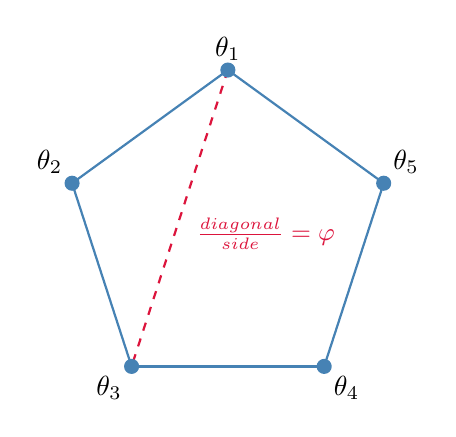
\begin{tikzpicture}[scale=1.6]
    % Pentagon vertices
    \foreach \i in {1,...,5} {
        \coordinate (p\i) at ({90+72*(\i-1)}:1.3);
    }
    
    % Draw edges
    \foreach \i [evaluate=\i as \j using {int(mod(\i,5)+1)}] in {1,...,5} {
        \draw[thick, bulkcolor] (p\i) -- (p\j);
    }
    
    % Draw one diagonal (showing golden ratio)
    \draw[dashed, anchorcolor, thick] (p1) -- (p3);
    
    % Vertices
    \foreach \i in {1,...,5} {
        \fill[bulkcolor] (p\i) circle (0.06);
    }
    
    % Labels
    \node[above] at (p1) {$\theta_1$};
    \node[above left] at (p2) {$\theta_2$};
    \node[below left] at (p3) {$\theta_3$};
    \node[below right] at (p4) {$\theta_4$};
    \node[above right] at (p5) {$\theta_5$};
    
    % Golden ratio annotation
    \node[anchorcolor, font=\small] at (0.3,0) {$\frac{diagonal}{side} = \varphi$};
\end{tikzpicture}
\caption{The cycle graph $C_5$ (regular pentagon). The diagonal-to-side ratio is $\varphi = (1+\sqrt{5})/2$.}
\label{fig:C5}
\end{figure}

\paragraph{Laplacian spectrum.} The discrete Laplacian $L_{C_5} = D - A$ (where $D$ is the degree matrix and $A$ the adjacency matrix) is a $5 \times 5$ circulant matrix with eigenvalues:
\begin{equation}
\lambda_k = 2 - 2\cos\!\left(\frac{2\pi k}{5}\right), \qquad k = 0, 1, 2, 3, 4
\label{eq:C5eigen}
\end{equation}
giving a doubly-degenerate spectrum:
\begin{equation}
\lambda_0 = 0, \qquad \lambda_1 = \frac{5-\sqrt{5}}{2} \approx 1.382~(\text{deg.}~2), \qquad \lambda_2 = \frac{5+\sqrt{5}}{2} \approx 3.618~(\text{deg.}~2)
\label{eq:C5eigenvals}
\end{equation}

\paragraph{Golden ratio emergence.} The ratio of non-zero eigenvalues:
\begin{equation}
\frac{\lambda_2}{\lambda_1} = \frac{5+\sqrt{5}}{5-\sqrt{5}} = \frac{(5+\sqrt{5})^2}{20} = \frac{30 + 10\sqrt{5}}{20} = \frac{3+\sqrt{5}}{2} = \varphi^2
\label{eq:golden}
\end{equation}
This is not numerology -- $\varphi^2$ is the unique spectral invariant of the regular pentagon, forced by $\mathbb{Z}_5$ symmetry. The identities $\lambda_1 + \lambda_2 = 5$, $\lambda_1 \lambda_2 = 5$, and $\varphi^2 = \varphi + 1$ all follow. Complete derivation in S1, Theorem~5.2 \cite{Hubka2026QSDsupp}.

\subsection{Graph Invariant Summary}

\begin{table}[h]
\centering
\begin{tabular}{lccccc}
\toprule
\textbf{Graph} & $|V|$ & $|E|$ & $\beta_1$ & $|\text{Aut}|$ & $\dim(\mathcal{H})$ \\
\midrule
$K_4$ (bulk) & 4 & 6 & 3 & 24 ($S_4$) & 16 \\
$C_5$ (code) & 5 & 5 & 1 & 10 ($D_5$) & 32 \\
\bottomrule
\end{tabular}
\caption{Topological invariants of the QSD graphs. Both are uniquely determined by the $[[5,1,3]]$ code.}
\label{tab:invariants}
\end{table}

%==============================================================================
\section{The Fundamental Constant Triad}
\label{sec:triad}
%==============================================================================

The $[[5,1,3]]$ code, through its graph structures $K_4$ and $C_5$, determines three fundamental constants. Together with $\Mpl$, they fix all QSD predictions.

\subsection{Holographic Bit Density: $\Hbfour$}

The exchange coupling $J$ in the Heisenberg Hamiltonian~\eqref{eq:HK4} is set by the maximum information throughput of each $K_4$ edge. Each edge is a quantum information channel bounded by the holographic principle: in $n$-dimensional spacetime, the information capacity per Planck area is $\Hbn = 1/(n \ln 2)$ bits.

\begin{theorem}[Holographic bit density]
\label{thm:hb4}
\begin{equation}
\boxed{J = \Hbfour = \frac{1}{|V(K_4)| \cdot \ln 2} = \frac{1}{4\ln 2} = 0.36067\ldots}
\label{eq:hb4}
\end{equation}
\end{theorem}

The ``4'' is $|V(K_4)| = n - k = 5 - 1$, the number of bulk qubits. In our universe, this equals the number of spacetime dimensions. This provides a code-theoretic explanation for the factor of~4 in the Bekenstein--Hawking formula $S_{\text{BH}} = A/(4\lp^2)$: the 4 arises from the 4~bulk qubits of the $[[5,1,3]]$ code, not as an unexplained numerical constant. Full proof in S1, Theorem~6.1 \cite{Hubka2026QSDsupp}.

\subsection{Geometric Strain: $\strain$}

The graphs $K_4$ (6 edges) and $C_5$ (5 edges) are structurally incompatible. The strain quantifies this mismatch.

\begin{definition}[Geometric strain]
\label{def:strain}
\begin{equation}
\boxed{\strain \equiv \frac{\beta_1(K_4)}{|\mathcal{H}_{K_4}| \times |V(C_5)| \times \varphi^2} = \frac{3}{16 \times 5 \times \varphi^2} = \frac{3}{80\varphi^2} = 0.014324\ldots}
\label{eq:strain}
\end{equation}
\end{definition}

Every factor is determined by the $[[5,1,3]]$ code: $\beta_1(K_4) = 3$ counts the independent cycles of the bulk graph (numerically equal to the code distance $d$), $|\mathcal{H}_{K_4}| = 2^{n-k} = 16$ is the syndrome Hilbert space dimension, $|V(C_5)| = n = 5$ is the block length, and $\varphi^2 = \lambda_2/\lambda_1$ is the spectral stiffness from the $C_5$ Laplacian. Physically, $\strain$ is the ratio of topological mismatch (what must be accommodated) to total capacity (what is available to absorb it).

The equivalent code-parameter form is $\strain = d/(2^{n-k} \cdot n \cdot \varphi^2)$. See S1, Definition~7.1 and Remark~7.3 for full discussion \cite{Hubka2026QSDsupp}.

\begin{remark}[Epistemic status of $\strain$]
\label{rem:strain_status}
The construction above is a \emph{geometric construction}: every ingredient is derived from the code, and the combination has a clear physical reading (cycles per capacity per stiffness). Other functions of the same code invariants would also be ``geometrically motivated.'' The specific combination is ultimately validated by its predictions (\S\ref{sec:couplings}). A first-principles derivation selecting this functional form uniquely remains an open problem.
\end{remark}

\subsection{Spectral Bond: $\specbond$}

Each $K_4$ edge carries an information-geometric ``charge'' combining the gauge geometry of the singlet channel with the spectral rigidity of $C_5$.

\begin{definition}[Spectral bond]
\label{def:specbond}
\begin{equation}
\boxed{\specbond \equiv \pi \varphi^2 = 8.2248\ldots}
\label{eq:specbond}
\end{equation}
\end{definition}

The factors: $\varphi^2 = \lambda_2/\lambda_1$ is the spectral stiffness of $C_5$ (Eq.~\ref{eq:golden}); $\pi$ is the $U(1)$ phase space factor from the gauge sector -- the singlet channel $\mathbf{1}$ in the edge decomposition $\mathbf{6} = \mathbf{1} \oplus \mathbf{2} \oplus \mathbf{3}$ carries $U(1)_Y$ gauge symmetry. The product combines continuous gauge geometry with discrete code spectrum.

\subsection{The Triad}

\begin{table}[h]
\centering
\begin{tabular}{ccll}
\toprule
\textbf{Constant} & \textbf{Value} & \textbf{Physical role} & \textbf{Status} \\
\midrule
$\Hbfour = 1/(4\ln 2)$ & 0.3607 & Information storage ($K_4$ exchange) & Derived \\
$\strain = 3/(80\varphi^2)$ & 0.01432 & Geometric strain ($K_4$--$C_5$ mismatch) & Constructed \\
$\specbond = \pi\varphi^2$ & 8.225 & Edge coupling (gauge $\times$ spectrum) & Derived \\
\bottomrule
\end{tabular}
\caption{The fundamental constant triad of QSD. Together with $\Mpl$ (experimental input), these determine all predictions.}
\label{tab:triad}
\end{table}

%==============================================================================
\section{Gauge Couplings from Graph Theory}
\label{sec:couplings}
%==============================================================================

We now present the central results of QSD: all three Standard Model gauge couplings derived from the code structure.

\subsection{The Fine Structure Constant}

\begin{theorem}[Tree-level $\alpha^{-1}$]
\label{thm:alpha_tree}
\begin{equation}
\alpha^{-1}_{\text{tree}} = \frac{|E(K_4)| \cdot \specbond}{\Hbfour} = \frac{6\specbond}{\Hbfour} = 24\pi\varphi^2\ln 2 = 136.824
\label{eq:alpha_tree}
\end{equation}
Each of the 6 edges of $K_4$ contributes one spectral bond $\specbond$ to the inverse electromagnetic coupling, normalised by the holographic bit density $\Hbfour$.
\end{theorem}

The $K_4$ graph has $\beta_1 = 3$ independent cycles, each generating one loop correction. The perturbation series terminates exactly after 3 terms (S4, \cite{Hubka2026QSDsupp}):
\begin{equation}
\alpha^{-1} = \frac{1}{\Hbfour}\!\left[6\specbond + 6\strain - 24\strain^2\varphi\!\left(1 + \frac{1}{\pi}\right)\right] = 137.033
\label{eq:alpha_full}
\end{equation}

\textbf{Accuracy}: 22~ppm compared to $\alpha^{-1}_{\text{exp}} = 137.036$ \cite{PDG2022}.

\begin{remark}[Why the series terminates]
Standard QFT renormalisation generates an infinite perturbation series. In QSD, the loop corrections arise from topological loads on the graph structure: $K_4$ has exactly $\beta_1 = 3$ independent cycles, and each generates one correction. There is no 4th independent cycle, so the series terminates. This is proved in S4, Theorem~1 \cite{Hubka2026QSDsupp}.
\end{remark}

\subsection{The Strong Coupling Constant}

\begin{theorem}[Strong coupling]
\label{thm:alpha_s}
\begin{equation}
\boxed{\alpha_s = \specbond \cdot \strain = \pi\varphi^2 \cdot \frac{3}{80\varphi^2} = \frac{3\pi}{80} = 0.11781}
\label{eq:alpha_s}
\end{equation}
\end{theorem}

Note the exact cancellation of $\varphi^2$: the golden ratio appears in both $\specbond$ (as a multiplicative factor) and $\strain$ (as an inverse factor), leaving $\alpha_s = 3\pi/80$ -- a pure expression in $\pi$ and the code integers 3 and 80.

\textbf{Accuracy}: 0.16\% compared to $\alpha_s^{\text{exp}}(M_Z) = 0.1180 \pm 0.0009$ \cite{PDG2022}.

\subsection{The Weak Mixing Angle}

\begin{theorem}[Weak mixing angle]
\label{thm:sin2theta}
\begin{equation}
\sin^2\theta_W = \frac{3}{13} + \frac{\strain}{32} = 0.23077 + 0.00045 = 0.23122
\label{eq:sin2theta}
\end{equation}
\end{theorem}

The tree-level value: the Standard Model gauge group has $N_{\text{gen}} = 8 + 3 + 1 + 1 = 13$ generators ($SU(3)_c + SU(2)_L + U(1)_Y$ plus trace normalisation). The weak sector contributes $\dim(SU(2)_L) = 3$, giving the ratio $3/13 = 0.23077$. The correction $\strain/32$ is a spectral perturbation from the full code Hilbert space ($\dim = 2^5 = 32$).

\textbf{Accuracy}: within experimental error of $\sin^2\theta_W^{\text{exp}} = 0.23122 \pm 0.00003$ \cite{PDG2022}.

\subsection{The Electromagnetic-Strong Identity}

\begin{theorem}[EM-strong duality]
\label{thm:em_strong}
An exact algebraic identity connects the electromagnetic and strong sectors:
\begin{equation}
\boxed{6\alpha_s = \alpha^{-1}_{\text{em,tree}} \times \Hbfour \times \strain}
\label{eq:em_strong}
\end{equation}
\end{theorem}

\begin{proof}
\begin{align}
\mathrm{LHS:\ } & 6\alpha_s = 6\specbond\strain = \color{red} 6\pi\varphi^2\strain \\
\mathrm{RHS:\ } & \alpha^{-1}_{\mathrm{tree}} \times \Hbfour \times \strain = (6\pi\varphi^2/\Hbfour) \times \Hbfour \times \strain = \color{red} 6\pi\varphi^2\strain 
\end{align}
\end{proof}

This identity holds to machine precision (verified to $10^{-16}$) and is a structural consequence of the graph theory, not a numerical coincidence. It expresses the fact that both $\alpha$ and $\alpha_s$ originate from the same spectral bond $\specbond$ acting on the same graph.

\subsection{Coupling Summary}

\begin{figure}[h]
\centering
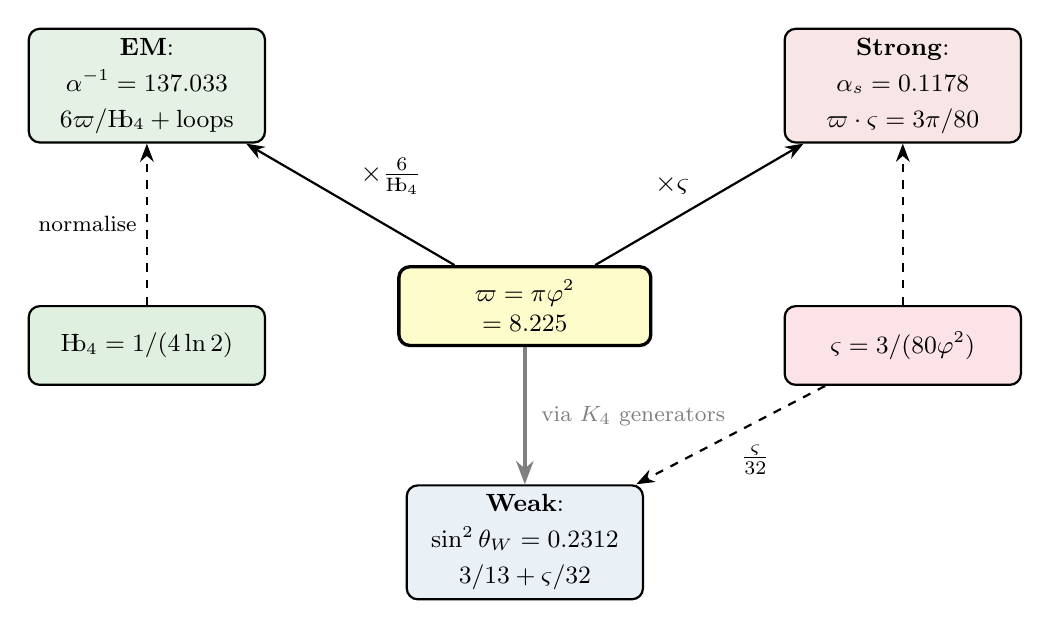
\begin{tikzpicture}[
    box/.style={draw, rounded corners, minimum width=3.0cm, minimum height=1.0cm,
                align=center, font=\small, thick},
    >=Stealth, thick
]
    % Central node — spectral bond
    \node[box, fill=yellow!20, very thick, minimum width=3.2cm] (sb) at (0,0)
        {$\specbond = \pi\varphi^2$\\$= 8.225$};

    % Three couplings
    \node[box, fill=u1color!12] (em) at (-4.8, 2.8)
        {\textbf{EM}:\\[2pt]$\alpha^{-1} = 137.033$\\[2pt]$6\specbond/\Hbfour + \text{loops}$};
    \node[box, fill=su3color!12] (strong) at (4.8, 2.8)
        {\textbf{Strong}:\\[2pt]$\alpha_s = 0.1178$\\[2pt]$\specbond \cdot \strain = 3\pi/80$};
    \node[box, fill=su2color!12] (weak) at (0, -3.0)
        {\textbf{Weak}:\\[2pt]$\sin^2\theta_W = 0.2312$\\[2pt]$3/13 + \strain/32$};

    % Supporting constants
    \node[box, fill=codegreen!12] (hb) at (-4.8, -0.5)
        {$\Hbfour = 1/(4\ln 2)$};
    \node[box, fill=anchorcolor!12] (strain) at (4.8, -0.5)
        {$\strain = 3/(80\varphi^2)$};

    % Arrows — primary flows
    \draw[->] (sb) -- (em) 
        node[midway, above right, font=\normalsize] {$\times \frac{6}{\Hbfour}$};
    \draw[->] (sb) -- (strong) 
        node[midway, above left, font=\normalsize] {$\times \strain$};
    \draw[->, very thick, gray] (sb) -- (weak)
        node[midway, right=2pt, font=\footnotesize] {via $K_4$ generators};

    % Arrows — supporting
    \draw[->, thick, dashed] (hb) -- (em)
        node[midway, left, font=\footnotesize] {normalise};
    \draw[->, thick, dashed] (strain) -- (strong);
    \draw[->, thick, dashed] (strain) -- (weak)
        node[midway, below right, font=\normalsize] {$\frac{\strain}{32}$};
\end{tikzpicture}
\caption{Flow from the fundamental triad $\{\Hbfour, \strain, \specbond\}$ to all three Standard Model gauge couplings.}
\label{fig:coupling_flow}
\end{figure}

%==============================================================================
\section{Energy Scale and Hierarchy}
\label{sec:hierarchy}
%==============================================================================

\subsection{The Hierarchy Problem}

The electroweak scale ($\sim 100$~GeV) is $\sim 10^{17}$ times smaller than the Planck scale ($10^{19}$~GeV). In the Standard Model, this requires fine-tuning to 17 decimal places. QSD explains this hierarchy as the information complexity of encoding the Standard Model in the $[[5,1,3]]$ code.

\subsection{The Information Reduction Factor}

\begin{theorem}[Emergence of $2^{-60}$]
\label{thm:hierarchy_factor}
The state space of the QSD code yields:
\begin{equation}
\mathcal{N} = \left(2^{n-k}\right)^{n(n-k-1)} = 16^{15} = 2^{60} \approx 1.15 \times 10^{18}
\label{eq:reduction}
\end{equation}
\end{theorem}

The $K_4$ Hilbert space has dimension $2^{n-k} = 16$. The interaction structure involves $n(n-k-1) = 5 \times 3 = 15$ independent channels ($n$ code positions times $\beta_1(K_4) = n - k - 1 = 3$ independent cycles). The total state space volume is $16^{15} = 2^{60}$.

\subsection{The Radion Mass}

The base energy scale $E_{\text{base}} = \Mpl / 2^{60}$ is enhanced by the geometric stiffness $\varphi^2$ and corrected by strain:

\begin{equation}
\boxed{\murad = \frac{\Mpl}{2^{60}} \times \varphi^2 \times (1 - 6\strain)}
\label{eq:radion}
\end{equation}

Numerically:
\begin{equation}
\murad = \frac{1.221 \times 10^{19}~\text{GeV}}{1.153 \times 10^{18}} \times 2.618 \times 0.914 = 25.34~\text{GeV}
\end{equation}

\begin{figure}[h]
\centering
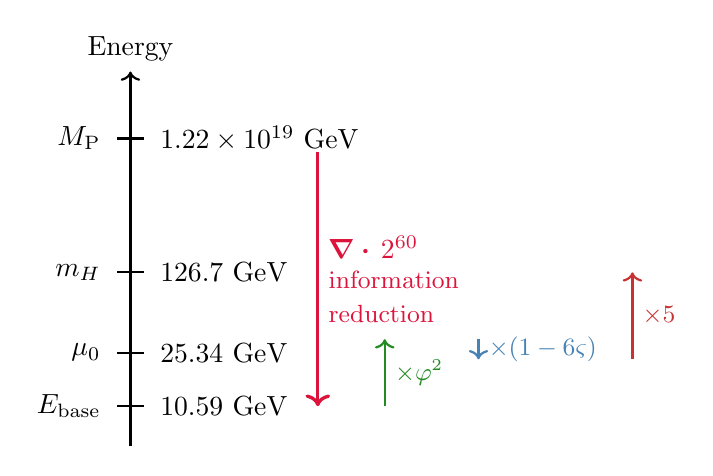
\begin{tikzpicture}[scale=0.85]
    % Energy axis
    \draw[thick, ->] (0,1.4) -- (0,7) node[above] {Energy};
    
    % Planck scale
    \draw[thick] (-0.2,6) -- (0.2,6);
    \node[left] at (-0.3,6) {$\Mpl$};
    \node[right] at (0.3,6) {$1.22 \times 10^{19}$ GeV};
    
    % Arrow: information reduction
    \draw[very thick, ->, anchorcolor] (2.8,5.8) -- (2.8,2) node[midway, right, text width=3cm] {$\div\, 2^{60}$ \\ \small information \\reduction};
    
    % Base scale
    \draw[thick] (-0.2,2) -- (0.2,2);
    \node[left] at (-0.3,2) {$E_{\text{base}}$};
    \node[right] at (0.3,2) {$10.59$ GeV};
    
    % Arrow: geometric enhancement
    \draw[thick, ->, u1color] (3.8,2) -- (3.8,3) node[midway, right] {\small $\times \varphi^2$};
    
    % Arrow: strain correction
    \draw[thick, ->, su2color] (5.2,3) -- (5.2,2.7) node[midway, right] {\small $\times(1-6\strain)$};
    
    % Radion scale
    \draw[thick] (-0.2,2.8) -- (0.2,2.8);
    \node[left] at (-0.3,2.8) {$\murad$};
    \node[right] at (0.3,2.8) {$25.34$ GeV};
    
    % Arrow: Higgs
    \draw[thick, ->, su3color] (7.5,2.7) -- (7.5,4) node[midway, right] {\small $\times 5$};
    
    % Higgs scale
    \draw[thick] (-0.2,4) -- (0.2,4);
    \node[left] at (-0.3,4) {$\mH$};
    \node[right] at (0.3,4) {$126.7$ GeV};
\end{tikzpicture}
\caption{The hierarchy of scales in QSD. The Planck mass is reduced by the information factor $2^{-60}$, enhanced by $\varphi^2$, strain-corrected to give the radion mass $\murad$, and multiplied by 5 (code length) to give the Higgs mass $\mH$.}
\label{fig:hierarchy}
\end{figure}

\subsection{The Higgs Mass}

The Higgs is the logical qubit of the $[[5,1,3]]$ code, a collective excitation of all 5 physical qubits:
\begin{equation}
\mH = 5 \times \murad = 5 \times 25.34 = 126.7~\text{GeV}
\label{eq:higgs}
\end{equation}

Compared to experiment ($\mH^{\text{exp}} = 125.1$~GeV): 1.3\% accuracy.

\subsection{Dimensionless Cross-Check}

QSD also gives an independent dimensionless VEV:
\begin{equation}
\nurad = \frac{\Hbfour}{\strain} = \frac{0.3607}{0.01432} = 25.18
\end{equation}
This is defined purely from information theory (no $\Mpl$), yet agrees with $\murad = 25.34$~GeV to 0.6\% -- a nontrivial consistency check.

%==============================================================================
\section{The QSD Action}
\label{sec:action}
%==============================================================================

The dynamics are governed by three sectors, each derived from the code structure:

\begin{equation}
S_{\text{QSD}} = \int dt \left[ \LL_{K_4} + \LL_{C_5} + \LL_{\text{topo}} \right]
\label{eq:action}
\end{equation}

\textbf{Heisenberg sector} (from $K_4$):
\begin{equation}
\LL_{K_4} = \hbar\Hbfour \sum_{i<j}^{4} \mathbf{S}_i \cdot \mathbf{S}_j
\end{equation}
governs spin exchange with coupling $J = \Hbfour$.

\textbf{Geometric sector} (from $C_5$):
\begin{equation}
\LL_{C_5} = \frac{\hbar}{2\omega}\dot{\theta}^2 - \hbar\omega(1 - \cos 5\theta)
\end{equation}
The $\mathbb{Z}_5$ symmetry of the stabilisers forces the $\cos 5\theta$ potential; this is derived from the continuum limit of the $C_5$ Laplacian, not assumed. The Mathieu equation emerges from graph geometry. See S3 \cite{Hubka2026QSDsupp}.

\textbf{Topological coupling} (Berry phase):
\begin{equation}
\LL_{\text{topo}} = \hbar \sum_{i=1}^{5} S_i^z \dot{\theta}_i
\end{equation}
When a spin traverses the $C_5$ cycle adiabatically, it acquires a Berry phase proportional to the solid angle subtended, generating this coupling.

The single dimensional parameter is $\hbar\omega = \murad = 25.34$~GeV.

\subsection{The Radion Field and Snap Mechanism}

The anchor qubit fluctuations define the radion field $\phi_r$ with a double-well potential:
\begin{equation}
V(\phi_r) = \frac{\lambda}{4}(\phi_r^2 - v_r^2)^2, \qquad v_r = \murad
\end{equation}

The ``snap'' is the phase transition where the anchor decouples from the bulk ($K_5 \to K_4 + \text{bit}$), releasing binding energy. This is the QSD mechanism for syndrome production. The radion couples to matter via the stress-energy trace: $\LL_{\text{int}} = -(\phi_r/v_r)\sum_f m_f \bar{\psi}_f \psi_f$, which gives mass-proportional branching ratios. Full Lagrangian derivation in S3 \cite{Hubka2026QSDsupp}.

%==============================================================================
\section{Phenomenology}
\label{sec:pheno}
%==============================================================================

\subsection{Syndrome Energy}

In quantum error correction, a syndrome is the measurement outcome revealing which error occurred. In QSD, syndromes are attempted but corrected violations of baryon number. When the anchor decouples, it releases binding energy from 4~severed bonds:

\begin{equation}
\Esyn = \murad(1 + 8\strain) = 25.34 \times 1.1146 = 28.24~\text{GeV}
\label{eq:syndrome}
\end{equation}

The factor $8\strain$ comes from 4~bonds $\times$ 2~endpoints, each contributing strain $\strain$.

CMS reported a dimuon excess near 28~GeV \cite{CMS2018dimuon}. QSD predicts 28.24~GeV -- agreement to 0.2\% with zero free parameters. The syndrome is not a particle but an error signal; it should appear as a broad, low-significance feature, not a narrow resonance. See S5 for detailed phenomenology \cite{Hubka2026QSDsupp}.

\subsection{Branching Ratios}

The mass-proportional coupling gives: $\text{BR}(b\bar{b}) = 94\%$, $\text{BR}(\tau^+\tau^-) = 5.7\%$, $\text{BR}(\mu^+\mu^-) = 0.02\%$. The experimental signature is dimuons near 28~GeV with associated $b$-jets.

\subsection{Proton Stability}

The $[[5,1,3]]$ code corrects all single-qubit errors; proton decay requires an uncorrectable error (2+ simultaneous qubit errors):
\begin{equation}
\tau_p \sim \frac{1}{\Punc} \sim \frac{1}{\strain^4} \sim 10^{38\text{--}40}~\text{years}
\label{eq:proton}
\end{equation}
safely above the current limit $\tau_p > 10^{34}$~years.

\subsection{Falsification Criteria}

\begin{table}[h]
\centering
\begin{tabular}{lcc}
\toprule
\textbf{Observable} & \textbf{QSD Prediction} & \textbf{Falsified if} \\
\midrule
Syndrome mass & $28.24 \pm 0.5$~GeV & Outside 27--29~GeV \\
Run~3 significance & $\leq 3$--$4\sigma$ & Exceeds $5\sigma$ \\
$\tau\tau/\mu\mu$ ratio & $\sim 300$ & Differs by $> 10\times$ \\
$b$-jet association & Required & Absent \\
Width & Broad/unresolved & Narrow resonance \\
Proton lifetime & $> 10^{38}$~yr & Observed decay \\
\bottomrule
\end{tabular}
\caption{Falsification criteria for QSD. If any prediction fails, the framework is ruled out.}
\label{tab:falsification}
\end{table}

The key prediction: the 28~GeV feature is real physics but will \emph{never} be discovered as a particle. If it reaches $5\sigma$, QSD is wrong.

%==============================================================================
\section{Open Problems}
\label{sec:open}
%==============================================================================

\subsection{Fermion Mass Hierarchy (Sketch)}

The fermion mass hierarchy should emerge from the $K_4$ spectrum and $S_4$ representation theory. The generation structure suggests:
\begin{equation}
m_f \sim c_f \times \murad \times \strain^{n_f}
\end{equation}
where $n_f$ is a generation index and $c_f$ is an $O(1)$ coefficient from the $S_4$ representation. Preliminary fits are consistent with observed masses, but the $c_f$ coefficients are not yet derived from first principles. The top quark ($n_f = 0$) lies near $\murad \times$~few, while lighter generations are exponentially suppressed by powers of $\strain \approx 0.014$.

This is the most important open problem in QSD: deriving the 6 quark and 6 lepton masses from the code structure without free parameters.

\subsection{Other Open Problems}

Several aspects of the Standard Model remain to be addressed: CP violation from code phases; neutrino masses from radion coupling; CKM/PMNS mixing matrices from $S_4$ representation theory; cosmological implications (dark matter candidates, inflationary dynamics); and a full derivation of the functional form of $\strain$ from first principles.

%==============================================================================
\section{Discussion and Conclusions}
\label{sec:discussion}
%==============================================================================

\subsection{What QSD Achieves}

Starting from a single axiom (the $[[5,1,3]]$ code) and one experimental input ($\Mpl$), QSD derives three gauge couplings, the electroweak hierarchy, the Higgs mass, and a collider prediction, all with zero free parameters. The results are summarised in Table~\ref{tab:summary}.

The framework is distinguished by two structural features. First, the perturbation series terminates exactly at 3~loops due to the topology of $K_4$ -- no divergences, no renormalisation ambiguities. Second, an exact algebraic identity (Eq.~\ref{eq:em_strong}) connects the electromagnetic and strong sectors, reflecting their common origin in the code.

\subsection{Relation to Other Approaches}

QSD shares goals with string theory (deriving SM parameters from geometry) but uses quantum information rather than extra dimensions. It shares discrete Planck-scale structure with loop quantum gravity and the information-theoretic perspective of holographic approaches \cite{Almheiri2015,Pastawski2015}. Unlike GUT models that begin with $SU(5)$ or $SO(10)$, QSD derives the gauge group $U(1)_Y \times SU(2)_L \times SU(3)_c$ from $S_4$ representation theory without postulating grand unification.

\subsection{Conclusion}

Quantum Spectrodynamics demonstrates that Standard Model parameters can be derived from the geometry of quantum error-correcting codes. The framework makes sharp, falsifiable predictions and is transparent about what is derived, what is constructed, and what remains open. If the programme succeeds, it suggests that the parameters of nature are not arbitrary but are fixed by the requirements of fault-tolerant quantum computation at the Planck scale.

%==============================================================================
% REFERENCES
%==============================================================================
\newpage
\bibliographystyle{unsrt}
\bibliography{QSD/common/qsd_references}

%==============================================================================
% APPENDICES
%==============================================================================
\newpage
\appendix

\section{Notation and Constants}
\label{app:notation}

\begin{table}[h]
\centering
\begin{tabular}{lll}
\toprule
\textbf{Symbol} & \textbf{Definition} & \textbf{Value} \\
\midrule
$\Hbfour$ & $1/(4\ln 2)$ & 0.3607 \\
$\strain$ & $\beta_1(K_4)/(|\mathcal{H}_{K_4}| \cdot |V(C_5)| \cdot \varphi^2) = 3/(80\varphi^2)$ & 0.01432 \\
$\specbond$ & $\pi\varphi^2$ & 8.225 \\
$\varphi$ & $(1+\sqrt{5})/2$ & 1.6180 \\
$\varphi^2$ & $(3+\sqrt{5})/2$ & 2.6180 \\
$\murad$ & $\Mpl / 2^{60} \times \varphi^2(1-6\strain)$ & 25.34~GeV \\
$\Esyn$ & $\murad(1+8\strain)$ & 28.24~GeV \\
$\mH$ & $5\murad$ & 126.7~GeV \\
$\Mpl$ & Planck mass & $1.221 \times 10^{19}$~GeV \\
\bottomrule
\end{tabular}
\caption{QSD notation and numerical values.}
\label{tab:notation}
\end{table}

\section{Mapping QSD to DCT Concepts}
\label{app:dct}

Quantum Spectrodynamics extends Dimensional Collapse Theory (DCT) \cite{Hubka2025DCT} from gravitational to particle physics. The central constant $\Hbfour = 1/(4\ln 2)$ has a natural interpretation in both frameworks: in DCT, it is the information density of the 2D ledger surface at a black hole horizon; in QSD, it is the exchange coupling of the $K_4$ Heisenberg Hamiltonian.

\begin{table}[h]
\centering
\begin{tabular}{ll}
\toprule
\textbf{DCT Concept} & \textbf{QSD Equivalent} \\
\midrule
Black hole horizon & Anchor--bulk boundary \\
Ledger (2D information surface) & Anchor qubit \\
Hawking radiation & Syndrome energy release \\
Information paradox resolution & Proton stability \\
Null-pair removal & Error detection \\
Dimensional collapse ($4 \to 2$) & Snap mechanism ($K_5 \to K_4 + \text{bit}$) \\
Unified Horizon Principle & Gauge coupling unification \\
$\Hbfour$ in entropy formula & $\Hbfour$ in Heisenberg coupling \\
Ledger radius $r_\LL$ & Radion VEV $\murad$ \\
\bottomrule
\end{tabular}
\caption{QSD--DCT dictionary. Both frameworks share $\Hbfour$ as the fundamental information-geometric constant.}
\label{tab:dct_dict}
\end{table}

The key physical insight connecting the two frameworks: Hawking radiation and LHC syndrome events are the same phenomenon at different scales -- the waste heat of information processing by the code.

\section{Axiom-to-Prediction Flow}
\label{app:flow}

\begin{center}
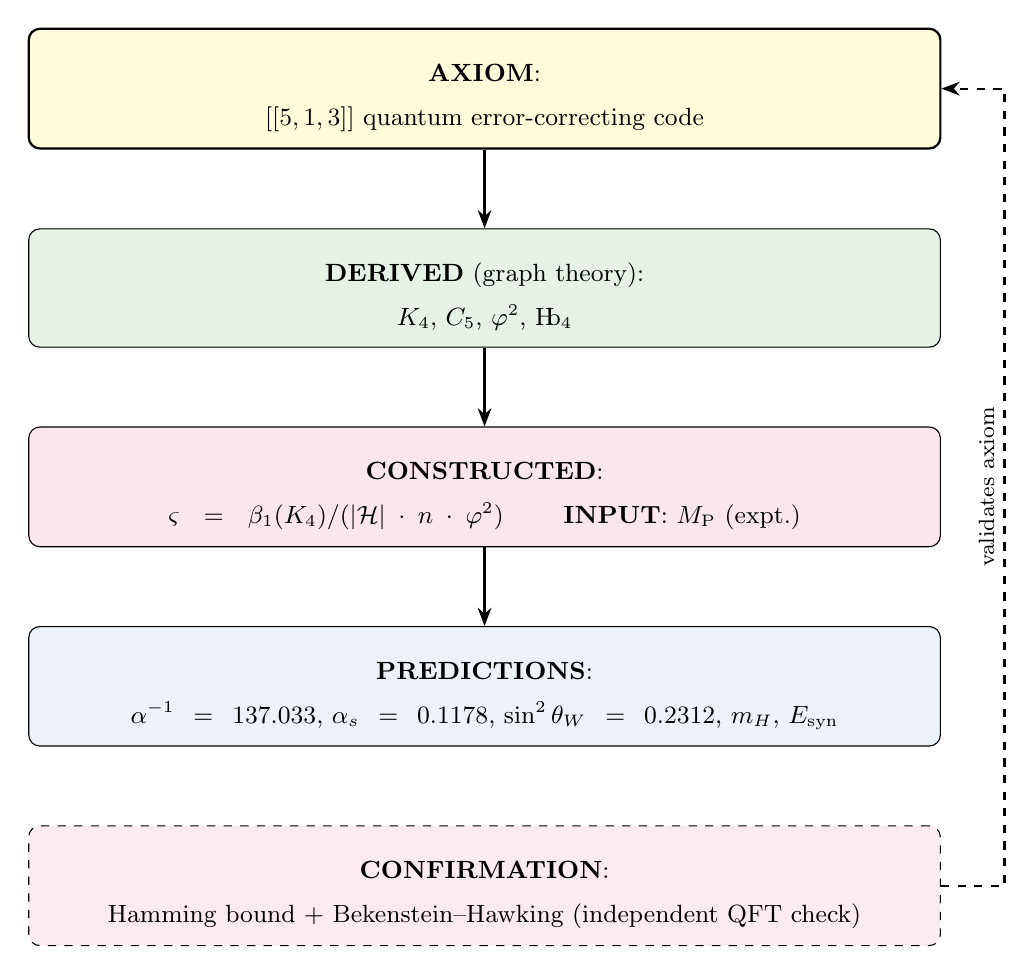
\begin{tikzpicture}[
  tier/.style={draw, rounded corners, align=center, font=\small,
               minimum height=1.25cm, text width=0.92\textwidth, inner sep=6pt},
  arrow/.style={-{Stealth}, thick},
  note/.style={font=\footnotesize},
  node distance=10mm,
]
  \usetikzlibrary{positioning,calc}

  \node[tier, fill=yellow!15, thick] (a)
    {\\[2pt]\textbf{AXIOM}:\\[5pt] $[[5,1,3]]$ quantum error-correcting code \\[2pt]};

  \node[tier, fill=codegreen!10, below=of a] (d1)
    {\\[2pt]\textbf{DERIVED} (graph theory):\\[5pt] $K_4$, $C_5$, $\varphi^2$, $\Hbfour$ \\[2pt]};

  \node[tier, fill=anchorcolor!10, below=of d1] (p)
    {\\[2pt]\textbf{CONSTRUCTED}:\\[5pt] $\strain = \beta_1(K_4)/(|\mathcal{H}| \cdot n \cdot \varphi^2)$
     \qquad \textbf{INPUT}: $\Mpl$ (expt.)\\[2pt]};

  \node[tier, fill=bulkcolor!10, below=of p] (r)
    {\\[2pt]\textbf{PREDICTIONS}:\\[5pt] $\alpha^{-1}=137.033$, $\alpha_s=0.1178$, $\sin^2\theta_W=0.2312$, $m_H$, $E_{\mathrm{syn}}$\\[2pt]};

  \node[tier, fill=purple!8, dashed, below=of r] (c)
    {\\[2pt]\textbf{CONFIRMATION}:\\[5pt] Hamming bound + Bekenstein--Hawking (independent QFT check)\\[2pt]};

  % Main pipeline (left spine)
  \draw[arrow] (a) -- (d1);
  \draw[arrow] (d1) -- (p);
  \draw[arrow] (p) -- (r);

    % Right-side loop back to axiom (tight corridor + vertical label)
\usetikzlibrary{calc}

\coordinate (loopX) at ($(a.east)+(8mm,0)$); % reduce if still too wide, e.g. 2mm

\draw[arrow, dashed]
  (c.east) -- ++(6pt,0) coordinate (s)                 % step out of the box
  -- ($(loopX |- s)$)                                  % go to corridor x at current y
  -- ($(loopX |- a.east)$)                              % go up to axiom y (vertical segment)
      node[midway, above, rotate=90, font=\footnotesize] {validates axiom}
  -- (a.east);                                         % go left into the axiom

\end{tikzpicture}
\end{center}

\end{document}
